\naslov{Introduction}

\begin{definition}
  Let $\Gamma$ be a graph with vertex set $\Omega$ and adjacency relation
  $\sim$.
  A permutation $g$ of $\Omega$ is an \pojem{automorphism} or a \pojem{symmetry}
  of $\Gamma$ if for any $u, v \in \Omega$, $u$ and $v$ are adjacent if and only if $u^g$
  and $v^g$ are adjacent.
\end{definition}

\begin{example}
  Consider the symmetries of the Petersen graph.
  The standard picture is invariant under rotations by a multiple of $2 \pi /
  5$, and by the $5$ reflections along a line through the origin and an outer
  vertex.
  We can describe these symmetries by permutations (labeling the vertices as in
  figure~\ref{fig:sg-01-petersen}):
  \begin{itemize}
  \item A one-step rotation in the negative direction is represented by
	\[
	  \rho = (1\,2\,3\,4\,5) (6\,7\,8\,9\,10).
	\]
	Then the other rotations are $\rho^2$, $\rho^3$, $\rho^4$ and $\rho^5 =
	\id$.
  \item The reflection around the vertical line is
	\[
	  \tau = (1) (2\,5) (3\,5) (6) (7\,10) (8\,9).
	\]
	We have more reflections, for example
	\[
	  \tau' = (2) (1\,3) (4\,5) (7) (6\,8) (9\,10).
	\]
  \end{itemize}
  The orbits of all the above described permutations are $\{1,2,3,4,5\}$ and
  $\{6,7,8,9,10\}$.
  But there is another automorphism,
  \[
	\sigma =
	\begin{pmatrix}
	  1 & 2 & 3  & 4 & 5 & 6 & 7 & 8 & 9 & 10 \\
	  6 & 8 & 10 & 7 & 9 & 1 & 3 & 5 & 2 & 4
	\end{pmatrix}
	= (1\,6) (2\,8\,5\,9) (3\,10\,4\,7)
  \]
  This permutation is of degree $4$.
  It in interesting to consider $\sigma^2$; it must map the outer cycle to the
  inner cycle, and vice versa, so it must be in $\sk{\rho, \tau}$.
  We can compute $\sigma^2 = \tau$.
  As it turns out, there is no symmetry of this graph which maps the outer cycle
  to the inner cycle, and vice versa, but is of order $2$.

  Consider also the conjugation $\rho^\sigma = \sigma^{-1} \rho \sigma$.
  We can compute $\rho^\sigma = \rho^2$.
  Since $\tau^\sigma = (\sigma^2)^\sigma = \tau$,
  \[
	\sk{\tau, \rho}^\sigma = \sk{\tau^\sigma, \rho^\sigma} = \sk{\tau, \rho^2}
	= \sk{\tau, \rho}
  \]
  and we have $\sk{\tau, \rho} \trianglelefteq H := \sk{\rho, \tau, \sigma}$ and
  $\sigma^2 \in \sk{\tau, \rho}$.
  So $\abs{H} = 2 \abs{\sk{\tau, \rho}} = 20$.
  But there are more automorphisms.

  We can relabel the vertices if the Petersen graph with elements of the set
  $\binom{[5]}{2}$ (note that for a set $S$, $\binom{S}{k}$ denotes the set of
  all $k$-subsets of $S$), as in figure~\ref{fig:sg-01-petersen-relabeled}.
  Note that $U, V \in \binom{[5]}{2}$ are connected if and only if they are
  disjoint (as sets).
  For any permutation $g \in S_5$, we can find a permutation $\alpha_g \in \Sym
  \binom{[5]}{2}$ which permutes the pairs by permuting their elements as $g$
  would.
  So there are at least $\abs{S_5} = 120$ automorphisms of the Petersen graph.
  Note that $g \mapsto \alpha_g$ is a group homomorphism.
\end{example}

\begin{figure*}[h!]
  \centering
  \begin{subfigure}{0.4\linewidth}
	\centering
	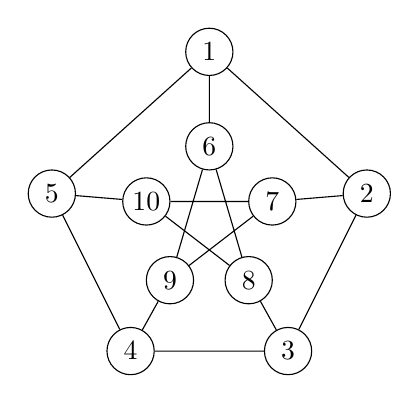
\begin{tikzpicture}
	  \node[draw,circle,minimum size=0.6cm,inner sep=0pt] (1) at (0,3.8) {1};
	  \node[draw,circle,minimum size=0.6cm,inner sep=0pt] (2) at (2,2) {2};
	  \node[draw,circle,minimum size=0.6cm,inner sep=0pt] (3) at (1,0) {3};
	  \node[draw,circle,minimum size=0.6cm,inner sep=0pt] (4) at (-1,0) {4};
	  \node[draw,circle,minimum size=0.6cm,inner sep=0pt] (5) at (-2,2) {5};
	  \node[draw,circle,minimum size=0.6cm,inner sep=0pt] (6) at (0,2.6) {6};
	  \node[draw,circle,minimum size=0.6cm,inner sep=0pt] (7) at (0.8,1.9) {7};
	  \node[draw,circle,minimum size=0.6cm,inner sep=0pt] (8) at (0.5,0.9) {8};
	  \node[draw,circle,minimum size=0.6cm,inner sep=0pt] (9) at (-0.5,0.9) {9};
	  \node[draw,circle,minimum size=0.6cm,inner sep=0pt] (10) at (-0.8,1.9) {10};

	  \draw (1) -- (2) -- (3) -- (4) -- (5) -- (1);
	  \draw (1) -- (6) (2) -- (7) (3) -- (8) (4) -- (9) (5) -- (10);
	  \draw (6) -- (8) -- (10) -- (7) -- (9) -- (6);
	\end{tikzpicture}
	\caption{The first labeling.}%
	\label{fig:sg-01-petersen}
  \end{subfigure}
  \begin{subfigure}{0.4\linewidth}
	\centering
	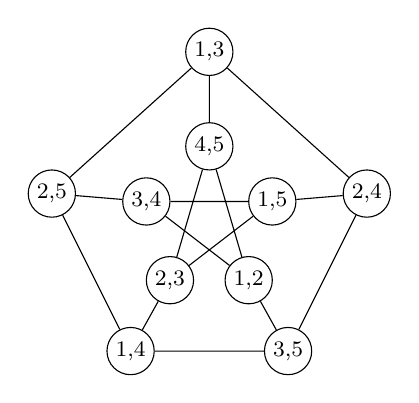
\begin{tikzpicture}
	  \node[draw,circle,minimum size=0.6cm,inner sep=0pt] (1) at (0,3.8) {\footnotesize 1,3};
	  \node[draw,circle,minimum size=0.6cm,inner sep=0pt] (2) at (2,2) {\footnotesize 2,4};
	  \node[draw,circle,minimum size=0.6cm,inner sep=0pt] (3) at (1,0) {\footnotesize 3,5};
	  \node[draw,circle,minimum size=0.6cm,inner sep=0pt] (4) at (-1,0) {\footnotesize 1,4};
	  \node[draw,circle,minimum size=0.6cm,inner sep=0pt] (5) at (-2,2) {\footnotesize 2,5};
	  \node[draw,circle,minimum size=0.6cm,inner sep=0pt] (6) at (0,2.6) {\footnotesize 4,5};
	  \node[draw,circle,minimum size=0.6cm,inner sep=0pt] (7) at (0.8,1.9) {\footnotesize 1,5};
	  \node[draw,circle,minimum size=0.6cm,inner sep=0pt] (8) at (0.5,0.9) {\footnotesize 1,2};
	  \node[draw,circle,minimum size=0.6cm,inner sep=0pt] (9) at (-0.5,0.9) {\footnotesize 2,3};
	  \node[draw,circle,minimum size=0.6cm,inner sep=0pt] (10) at (-0.8,1.9) {\footnotesize 3,4};

	  \draw (1) -- (2) -- (3) -- (4) -- (5) -- (1);
	  \draw (1) -- (6) (2) -- (7) (3) -- (8) (4) -- (9) (5) -- (10);
	  \draw (6) -- (8) -- (10) -- (7) -- (9) -- (6);
	\end{tikzpicture}
	\caption{The second ordering}%
	\label{fig:sg-01-petersen-relabeled}
  \end{subfigure}
  \caption{The Petersen graph}
\end{figure*}

\begin{definition}
  Let $\Omega$ be a nonempty finite set.
  A \pojem{permutation} on $\Omega$ is a bijection $\Omega \to \Omega$.
  We denote the set of all permutations of $\Omega$ with $\Sym \Omega$, or
  $S_n$, if $\Omega = [n]$.
\end{definition}

\begin{definition}
  If $g \in \Sym \Omega$ and $\omega \in \Omega$, then $\omega^g = g(\omega)$
  denotes the application of $g$ on $\omega$.
\end{definition}

\begin{definition}
  The composition of two permutations $g, h \in \Sym \Omega$ is defined as the
  permutation which acts as
  \[
	g \circ h: \omega \to g(h(\omega)) = {(\omega^h)}^g.
  \]
\end{definition}

We introduce the inverse composition as our product operation on $\Sym \Omega$,
defined as
\[
  gh = h \circ g.
\]
Then $\omega^{(g h)} = {(\omega^g)}^h =: \omega^{gh}$.
Note that both $(\Sym \Omega, \circ)$ and $(\Sym \Omega, \cdot)$ are groups, and
they are different groups, but they are isomorphic.

\begin{definition}
  We denote the set of all transpositions of $\Omega$ with $T_\Omega$.
\end{definition}

\begin{remark}
  Note that $\sk{T_\Omega} = \Sym \Omega$.
\end{remark}

\begin{definition}
  Denote by $\Alt \Omega$ the set of all even permutations of $\Omega$.
\end{definition}

\begin{remark}
  This is an index-$2$ normal subgroup in $\Sym \Omega$.
\end{remark}

\begin{definition}
  The \pojem{cyclic} group of order $n$ is $\Cyc(n) =
  \sk{(1\,2\,3\,\ldots\,n)} \le S_n$.
\end{definition}

\begin{definition}
  The \pojem{dihedral} group of order $n$ is
  \[
	\Dih(n) =
	\begin{cases}
	  \sk{(1\,2\,3\,\ldots\,n), (1) (2,n) (3,n-1) \ldots
	  (\frac{n}{2},\frac{n+2}{2})} & \text{$n$ even} \\
	  \sk{ (1\,2\,3\,\ldots\,n), (1) (2,n-1) \ldots
	  (\frac{n+1}{2},\frac{n+3}{2}) } & \text{$n$ odd}
	\end{cases}
  \]
  as a subgroup of $S_n$.
\end{definition}

\begin{remark}
  This is the automorphism group of a cyclic graph on $n$ vertices.
\end{remark}

\begin{definition}
  Let $G$ be an abstract group and $\Omega$ a set.
  A \pojem{group action} is a group homomorphism $\rho: G \to \Sym \Omega$.
\end{definition}

\begin{remark}
  We often write $\omega^g$ when we really mean $\omega^{\rho(g)}$.
\end{remark}

\begin{remark}
  As a shorthand, we can write $\rho(g) = g^\Omega$, and $G^\Omega = \rho(G) =
  \{ g^\Omega \such g \in G \}$.
\end{remark}

\begin{definition}
  An action is \pojem{faithful} if the kernel of the action is trivial.
\end{definition}

\begin{remark}
  Note that $G^\Omega = \im \rho \cong G / \jedro \rho$.
\end{remark}

\begin{remark}
  Any faithful action is an isomorphism $G \to G^\Omega$, so we may view $G$ as
  a subgroup in $\Sym \Omega$.
  So $G$ becomes a permutation group.
\end{remark}

\begin{definition}
  The \pojem{point stabiliser} of an element $\omega \in \Omega$ is the subgroup
  $G_\omega = \{ g \in G \such \omega^g = \omega \}$.
\end{definition}

\begin{definition}
  The \pojem{set stabiliser} $G_\Delta$ of a subset $\Delta \subseteq \Omega$ is
  the subgroup $G_\Delta = \{ g \in G \such \Delta^g = \Delta \}$.
\end{definition}

\begin{definition}
  The \pojem{point-wise stabiliser} $G_{(\Delta)}$ of a subset $\Delta \subseteq
  \Omega$ is the subgroup $G_{(\Delta)} = \bigcap_{\omega \in \Delta} G_\omega$.
\end{definition}

\begin{remark}
  Note that $G_\Delta$ has an induced action on $\Delta$.
  But even if the action of $G$ on $\Delta$ is faithful, $G_\Delta$ might act on
  $\Delta$ unfaithfully.
  If we label the induced permutation group with $G_\Delta^\Delta$, then we have
  \[
	G_\Delta^\Delta \cong G_\Delta / G_{(\Delta)}.
  \]
\end{remark}

\begin{definition}
  The \pojem{orbit} of a point $\omega \in \Omega$ is the set $\omega^G = \{
  \omega^g \such g \in G \}$.
  We label $\Omega / G = \{ \omega^g \such \omega \in \Omega \}$.
\end{definition}

\begin{remark}
  The set $\Omega / G$ is a partition of $\Omega$ into disjoint sets.
\end{remark}

\begin{definition}
  A group $G$ acts \pojem{transitively} on $\Omega$ if $\abs{\Omega / G} = 1$.
\end{definition}

\begin{lemma}
  Let $G$ act on $\Omega$ faithfully and let $\Omega_1, \ldots, \Omega_r$ be the
  orbits of this action.
  Then we can embed $G$ into the group $G^{\Omega_1} \times \cdots \times
  G^{\Omega_r}$.
  Additionally, if $\pi_i : G^{\Omega_1} \times \cdots \times G^{\Omega_r} \to
  G^{\Omega_i}$ is the canonical projection, then the composition of $\pi_i$ and
  the embedding is surjective.
\end{lemma}

\begin{remark}
  We call $G^{\Omega_1}, \ldots, G^{\Omega_r}$ the \pojem{transitive
	constituents}.
\end{remark}

\begin{remark}
  In this case, we say that $G$ is a \pojem{subdirect product} of $G^{\Omega_1},
  \ldots, G^{\Omega_r}$ (it is a subset of a direct product).
\end{remark}

\begin{lemma}[orbit-stabiliser]
  If $G$ acts on $\Omega$ and $\omega \in \Omega$, then $\abs{G} =
  \abs{G_\omega} \cdot \abs{\omega^G}$.
\end{lemma}

\begin{definition}
  Let $g \in G$.
  Then $\Fix_\Omega(g) = \{ \omega \in \Omega \such \omega^g = \omega \}$ is the
  set of fixed points of $g$, and $\Supp_\Omega(g) = \Omega \setminus
  \Fix_\Omega(g)$.
\end{definition}

\begin{lemma}[Cauchy-Frobenius / the lemma that is not Burnside's]
  Let $G$ act on $\Omega$.
  Then
  \[
	\abs{\Omega / G} = \inv{\abs{G}} \sum_{g \in G} \Fix_\Omega(g).
  \]
\end{lemma}

\begin{corollary}
  If $G$ acts transitively on $\Omega$, then it contains an element that fixes
  no points.
\end{corollary}

\begin{remark}
  We call such elements \pojem{derangements}.
\end{remark}

\begin{definition}
  An action $\rho$ is \pojem{regular} if it is transitive and the stabiliser of
  a point is trivial.
\end{definition}

\begin{remark}
  If an action is regular, then the stabiliser of every point is trivial.
\end{remark}

\begin{example}[action by right multiplication]
  Let $G$ be a group.
  Define $\Omega = G$ and for $g, h \in G$, $h^g := h g$.
  This is a regular action.
\end{example}

\begin{example}[action by left multiplication]
  Let $G$ be a group.
  Define $\Omega = G$ and for $g, h \in G$, $h^g := g^{-1} h$.
  This is also a regular action.
\end{example}

\begin{remark}
  All regular actions are isomorphic to one another.
\end{remark}

\begin{example}[action by conjugation]
  Again set $\Omega = G$ and for $g, h \in G$, define $h^g = g^{-1} h g$.
  The stabiliser of a point $h$ is precisely the centraliser of $h$ in the
  group, i.e.~the elements of $G$ which commute with $h$.
  The kernel of this action is
  \[
	\bigcap_{h \in G} G_h = \bigcap_{h \in G} C_G(h) = Z(G).
  \]
  This action is then faithful if and only if the center is trivial.
\end{example}

\begin{example}[action on subgroups]
  Let $\Omega = S(G) = \{ H \such H \le G \}$ be the set of all subgroups of
  $G$.
  Then define $H^g = g^{-1} H g$.
  The centraliser of $H$ is precisely the normaliser of $H$ in $G$.
\end{example}

\begin{example}[action on Sylow subgroups]
  Let $G$ be a group with $\abs{G} = p^e m$ where $p \in \Prime$, $e \in \N$ and
  $p$ does not divide $m$.
  Let $\Syl_p(G)$ be the set of all Sylow $p$-subgroups of $G$.
  If we take $\Omega = \Syl_p(G)$, then we can introduce $P^g = g^{-1} P g$.
  This action is transitive.
\end{example}

\begin{example}[action on cosets]
  Let $H \le G$ be a subgroup of $G$.
  Take $\Omega = G / H$ be the set of left cosets of $H$, and introduce the
  action $(Hh)^g = H(hg)$.
  If $Hh = Hk$, then $hk^{-1} \in H$, so also $hgg^{-1}k \in H$, which means
  this action is well-defined.
  We can compute that the stabiliser of a coset $H x$ is precisely $x^{-1} H x$.

  The kernel of the action is the intersection of all the stabilisers, which is
  the largest subgroup of $H$ that is normal in $G$.
  This is called the \pojem{core} of $H$.
  So the action is faithful if and only if the core of $H$ is trivial, so if and
  only if $H$ contains no nontrivial normal subgroups of $G$.
\end{example}

\begin{lemma}
  Let $G$ act on $\Omega$ and let $\omega \in \Omega, x \in G$.
  Then
  \[
	G_{\omega^x} = (G_\omega)^x,
  \]
  where the superscript on the left denotes the action on $\Omega$, and the
  superscript on the right is the conjugation by $x$.
\end{lemma}

\begin{proof}
  Let $g \in G_{\omega^x}$.
  Then $(\omega^x)^g = \omega^x$, which is equivalent to $\omega^{xg} =
  \omega^x$, which is again equivalent to $\omega^{x g x^{-1}} = \omega$, so $xg
  x^{-1} \in G_\omega$ or $g \in (G_\omega)^x$.
\end{proof}

\begin{example}
  Let $k \in \N$. We label $\Omega^{\{k\}} = \binom{\Omega}{k}$. If $G$ acts on
  $\Omega$, then we have an induced action of $G$ on $\Omega^{\{k\}}$, by $X^g =
  \{ x^g \such x \in X \}$.
  More generally, $G$ acts on the power set $P(\Omega)$ by the same rule.
  This action preserves cardinality.
\end{example}

% LocalWords:  subdirect Frobenius Sylow
